% You can easily modify this theme by either changing
% the main color specified below in lines 11 and 12 
% or exchan ging the background picture located at 
% ./style/background.png!

%%%%% NEEDS TO BE COMPILED WITH LuaLaTeX %%%%%

% --------------------------------------------------

\documentclass[aspectratio=169,11pt,dvipsnames, handout]{beamer} 
\definecolor{defaultclr}{HTML}{114F66} 
\definecolor{secondclr}{HTML}{994C9E} 
% Colors ------------------------------------------------------

\usecolortheme[named=defaultclr]{structure}


% Packages ----------------------------------------------------

\usetheme{Frankfurt}
\usepackage[gen]{eurosym}
\usepackage{tcolorbox}
\usepackage{amsmath, amssymb}
\usepackage{csquotes}
\MakeOuterQuote{"}
\usepackage{soul}
%\usepackage{parskip}
%\setlength{\parskip}{\smallskipamount} 

% Add setspace package if desired
\usepackage{setspace}
\onehalfspacing

\usepackage{tikz}
\usetikzlibrary{fadings}
\usetikzlibrary{shadings}
\usetikzlibrary{patterns}
\usepackage{transparent}
\usepackage{xcolor}
\usepackage{gradient-text}
\PassOptionsToPackage{silent}{fontspec} 
\usepackage{lipsum}
\usepackage{booktabs}
\usepackage{colortbl}
\usepackage{adjustbox}
\usepackage{tabularx}

\usepackage{svg}




% Links -------------------------------------------------------

\hypersetup{
    colorlinks,
    allcolors=.,
    urlcolor=defaultclr,
    citecolor=defaultclr
}


% References --------------------------------------------------

\usepackage[%
backend=biber,%
style=apa,%
sorting=nyt,%
]{biblatex}
\DeclareFieldFormat{apacase}{#1}
\setbeamertemplate{bibliography item}{}
\addbibresource{references.bib}

\renewcommand*{\bibfont}{\normalfont\footnotesize}

\usepackage{xparse}

% Small, grey parencite
\let\originalparencite\parencite
\RenewDocumentCommand{\parencite}{O{} O{} m}{%
  {\footnotesize\textcolor{gray}{\originalparencite[#1][#2]{#3}}}%
}



% Fonts -------------------------------------------------------

\usepackage{unicode-math}

\setmainfont[%
    Path=./style/,%
    Extension=.ttf,%
    Scale=1.0,%
    UprightFont=*-Regular,%
    BoldFont=*-Bold,%
    ItalicFont=*-Italic,%
    BoldItalicFont=*-BoldItalic%
]{Inter}

\setsansfont[%
    Path=./style/,%
    Extension=.ttf,%
    Scale=1.0,%
    UprightFont=*-Regular,%
    BoldFont=*-Bold,%
    ItalicFont=*-Italic,%
    BoldItalicFont=*-BoldItalic%
]{Inter}

\newfontfamily{\titlefont}{RedHatDisplay}[%
    Path=./style/,%
    Extension = .ttf,%
    Scale=1.0,%
    UprightFont=*-Regular,%
    BoldFont=*-Bold,%
    ItalicFont=*-Italic,%
    BoldItalicFont=*-BoldItalic%
    ]

\newfontfamily{\interfont}{Inter}[%
    Path=./style/,%
    Extension = .ttf,%
    Scale=1.0,%
    UprightFont=*-Regular,%
    BoldFont=*-Bold,%
    ItalicFont=*-Italic,%
    BoldItalicFont=*-BoldItalic%
    ]
    
\setmathfont{Fira Math}

\setmathfont[Path=./style/, Scale=0.9, range={up}]{Inter-Regular.ttf}
\setmathfont[Path=./style/, Scale=0.9, range={it}]{Inter-Italic.ttf}
\setmathfont[Path=./style/, Scale=0.9, range={bfup}]{Inter-Bold.ttf}
\setmathfont[Path=./style/, Scale=0.9, range={bfit}]{Inter-BoldItalic.ttf}

% Do NOT load the real bm package!
\let\bm\symbfit



% Beamer Templates --------------------------------------------

%\setbeamertemplate{frametitle}[default][center]

\setbeamercolor{frametitle}{parent=subsection in head/foot}
\setbeamercolor{frametitle right}{parent=section in head/foot}
\setbeamercolor{footnote}{fg=gray} % I am setting all footnotes to appear in gray

\makeatletter
\pgfdeclarehorizontalshading[frametitle.bg,frametitle right.bg]{beamer@frametitleshade}{\paperheight}{%
    color(0pt)=(frametitle.bg);
    color(\paperwidth)=(frametitle right.bg)}


\setbeamertemplate{frametitle}
{%
    \nointerlineskip%
    \vskip-2pt%
    \hbox{\leavevmode
        \advance\beamer@leftmargin by -12bp%
        \advance\beamer@rightmargin by -12bp%
        \beamer@tempdim=\textwidth%
        \advance\beamer@tempdim by \beamer@leftmargin%
        \advance\beamer@tempdim by \beamer@rightmargin%
        \hskip-\Gm@lmargin%
        \hbox{%
            \setbox\beamer@tempbox=\hbox{%
                \begin{minipage}[b]{\paperwidth}%
                    \vbox{}\vskip-.75ex%
                    \centering
                    \insertframetitle%
                    \ifx\insertframesubtitle\@empty%
                    \strut\par%
                    \else
                    \par{\usebeamerfont*{framesubtitle}{\usebeamercolor[fg]{framesubtitle}\insertframesubtitle}\strut\par}%
                    \fi%
                    \vskip4pt%
                    \nointerlineskip
                    \vbox{}%
                \end{minipage}%
            }%
            \beamer@tempdim=\ht\beamer@tempbox%
            \advance\beamer@tempdim by 6pt%
            \begin{pgfpicture}{0pt}{0pt}{\paperwidth}{\beamer@tempdim}%
                \usebeamercolor{frametitle right}%
                \pgfpathrectangle{\pgfpointorigin}{\pgfpoint{\paperwidth}{\beamer@tempdim}}%
                \pgfusepath{clip}%
                \pgftext[left,base]{\pgfuseshading{beamer@frametitleshade}}%
            \end{pgfpicture}%
            \hskip-\paperwidth%
            \box\beamer@tempbox%
        }%
        \hskip-\Gm@rmargin%
    }%
    \nointerlineskip%
    \vskip-0.2pt%
    \vskip-2pt%
}


\makeatother

\setbeamercolor{section in toc}{fg=red}
%%%

\colorlet{titleleft}{defaultclr}
\colorlet{titleright}{defaultclr}

\setbeamercolor*{frametitle}{fg=white}

\makeatletter
\pgfdeclarehorizontalshading[titleleft,titleright]{beamer@frametitleshade}{\paperheight}{%
    color(-0.25\paperwidth)=(titleleft);
    color(1.25\paperwidth)=(titleright)}
\makeatother

\setbeamerfont{frametitle}{series=\bfseries, family = \titlefont}
\setbeamerfont{title}{size = \Huge, series=\bfseries, family = \titlefont}
\setbeamerfont{headline}{size=\scriptsize, family = \titlefont}
\setbeamercolor{title}{fg=defaultclr!50!black}

\setbeamersize{text margin left=5.3mm,text margin right=5.3mm} 

\beamertemplatenavigationsymbolsempty
\setbeamertemplate{headline}{}

\setbeamercolor{titlelike}{parent=structure}

\addtobeamertemplate{navigation symbols}{}{%
    \usebeamerfont{footline}%
    \usebeamercolor[fg]{footline}%
    \hspace{1em}%
    \insertframenumber/\inserttotalframenumber
}

\setbeamertemplate{itemize/enumerate subbody begin}{\small}

\setbeamertemplate{itemize item}[circle]
\setbeamertemplate{itemize subitem}[circle]
\setbeamertemplate{itemize subsubitem}[circle]

\setbeamertemplate{enumerate items}[default]

% Section Headers --------------------------------------------

\setbeamertemplate{section in toc}{\inserttocsection}
\setbeamerfont{section in toc}{size=\huge,series=\bfseries,family=\titlefont}

\AtBeginSection[]
{{\setbeamercolor{section in toc}{bg=white, fg=white}
\setbeamercolor{section in toc shaded}{bg=gray, fg=gray}
\setbeamerfont{section in toc shaded}{size=\small}
%\setbeamercolor{background canvas}{bg=structure}
\setbeamertemplate{background canvas}{%
\begin{tikzpicture}[remember picture,overlay]
\shade[inner color=defaultclr, outer color=defaultclr]
    ([shift={(-5cm,5cm)}]current page.center) circle [radius=1.25\paperwidth];
\end{tikzpicture}%     
}

  \begin{frame}\centering
    \bfseries\color{white}\tableofcontents[currentsection]
  \end{frame}}}


% Miscellaneous ----------------------------------------------

\newcommand{\ind}{\perp\!\!\!\!\perp} 

\newcommand{\mathcolorbox}[2][yellow]{\mathchoice%
  {\colorbox{#1}{$\displaystyle#2$}}%
  {\colorbox{#1}{$\textstyle#2$}}%
  {\colorbox{#1}{$\scriptstyle#2$}}%
  {\colorbox{#1}{$\scriptscriptstyle#2$}}}%

\renewcommand{\arraystretch}{0.68}

% Redefine how the continuation of frametitles is displayed
\makeatletter
\defbeamertemplate{frametitle continuation}{custom}[1][]
{(\insertcontinuationcount)}
\makeatother
\setbeamertemplate{frametitle continuation}[custom]

% Tight Font
\newcommand{\tightfont}{%
  \setlength{\spaceskip}{
    0.3\fontdimen2\font
    plus 0.3\fontdimen2\font
    minus 0.3\fontdimen3\font
  }%
}
% Setup for notes
%\setbeameroption{show notes on second screen=right}

\definecolor{upcol}{HTML}{C160CC}
\definecolor{downcol}{HTML}{D48300}


% ---------------------------------------------------
% TITLE
% ---------------------------------------------------

\title{Mines — Rivers — Yields}
\subtitle{Downstream Mining Impacts on Agriculture in Africa}
\author{Lukas Vashold~(\href{mailto:lukas.vashold@wu.ac.at}{lukas.vashold@wu.ac.at}) \\ Gustav Pirich~(\href{mailto:gustav.pirich@wu.ac.at}{gustav.pirich@wu.ac.at}) \\ \textbf{Max Heinze}~(\href{mailto:maximilian.heinze@wu.ac.at}{maximilian.heinze@wu.ac.at}) \\ Nikolas Kuschnig~(\href{mailto:nikolas.kuschnig@wu.ac.at}{nikolas.kuschnig@wu.ac.at})}
\institute{NOeG Winter Workshop}
\date{December 18, 2024}

% ---------------------------------------------------
% BODY
% ---------------------------------------------------

\begin{document}	

% ---------------------------------------------------
{
\setbeamertemplate{background canvas}{%
\begin{tikzpicture}[remember picture,overlay]
\shade[inner color=defaultclr!10, outer color=defaultclr!10]
    ([shift={(-5cm,5cm)}]current page.center) circle [radius=1.25\paperwidth];
\end{tikzpicture}%     
}
\begin{frame}[plain]

\maketitle

\vspace{-3em}
%\hspace{0.5em}\includegraphics<beamer>[width=7em]{slidesdownload.png} 

\vspace{-0.5em}

%\onslide<beamer>{Download Slides}

\end{frame}
}

% ---------------------------------------------------

\section{Background}

% ---------------------------------------------------


\begin{frame}{Mines — Curse or Blessing?}
\vspace{-2.5em}
    \begin{columns}[t]
        \begin{column}{0.45\textwidth}
            \begin{tcolorbox}[colback=defaultclr!20, colframe=defaultclr!20, fontupper=\bfseries\color{defaultclr!40!black}, width=\textwidth, sharp corners, boxrule=0pt, halign=center]
                \textbf{A Blessing?}
            \end{tcolorbox}
            \vspace{-0.75em}
            \begin{itemize}
                \item Demand for relevant \textbf{minerals} is projected to increase \textbf{fourfold} until 2050 \parencite{hund2023}.
                \vspace{0.5em}\item \colorbox{defaultclr!15}{\bfseries Extraction Benefits} include:
        \begin{itemize}
            \item enabling the \textbf{green transition},
            \item increasing local \textbf{incomes} \parencite{bazillier2020},
            \item and improving \textbf{wealth} and \textbf{asset ownership} \parencite{vondergoltz2019}.
        \end{itemize}
            \end{itemize}
        \end{column}
        \begin{column}{0.45\textwidth}
            \begin{tcolorbox}[colback=secondclr!20, colframe=secondclr!20, fontupper=\bfseries\color{secondclr!40!black}, width=\textwidth, sharp corners, boxrule=0pt, halign=center]
                \textbf{A\phantom{j}Curse?}
            \end{tcolorbox}
            \setbeamercolor{itemize item}{fg=secondclr}
            \setbeamercolor{itemize subitem}{fg=secondclr}
            \vspace{-0.75em}
            \begin{itemize}
                \item Resource extraction causes \textbf{negative externalities.}
                \item \colorbox{secondclr!15}{\bfseries Ecological effects} include:
                \begin{itemize}
            \item Mines \textbf{use water} and produce \textbf{sediments and tailings} \parencite{moura2022}.
            \item Pollutants include \textbf{mercury} and \textbf{lead} \parencite{schwarzenbach2010}.
            \item Industrial pollution \textbf{harms plant growth} \parencite{Yang2021}.
        \end{itemize}
            \end{itemize}
            \setbeamercolor{itemize item}{fg=defaultclr}
            \setbeamercolor{itemize subitem}{fg=defaultclr}
        \end{column}
    \end{columns}
\end{frame}


% ---------------------------------------------------


\begin{frame}{How to Find Affected Areas}
\label{frame:intro}
    \begin{columns}
        \begin{column}{0.35\linewidth}
            \includegraphics[height=0.9\paperheight]{img/basins.pdf}
        \end{column}
        \begin{column}{0.65\linewidth}
            Using data on \textbf{river basins} \parencite{lehner2013}, we know where water flows from a given location.

            \vspace{1em}
            
            Water moves from \colorbox{upcol!30}{\bfseries upstream} to \colorbox{downcol!30}{\bfseries downstream} of a mine.

            \vspace{1em}
        
            Using a \textbf{remotely-sensed vegetation index}, we find evidence for less healthy vegetation \colorbox{downcol!30}{\bfseries downstream}.

            \vspace{1em}\flushright

            \hyperlink{frame:appintro}{\beamerbutton{\bfseries show schematic depiction}}
            \hyperlink{frame:appbasins}{\beamerbutton{\bfseries show more on basins}}
        \end{column}
    \end{columns}
\end{frame}


% ---------------------------------------------------

\begin{frame}{Research Question}

\begin{tcolorbox}[colback=secondclr!20, colframe=secondclr!20, fontupper=\bfseries\color{secondclr!40!black}, width=\textwidth, sharp corners, boxrule=0pt, halign=center]
\bfseries What is the causal effect of water pollution from mining on agricultural productivity in Africa?
\end{tcolorbox}

\vspace{1em}

    \begin{itemize}
        \item \textbf{Africa} is a particularly interesting focus because
        \vspace{0.5em}
        \begin{itemize}
            \item it has a \textbf{booming mining industry} \parencite{icmm2022},
            \vspace{0.25em}
            \item with many \textbf{artisanal and small-scale mines} \parencite{asm2022, girard2022}
            \vspace{0.25em}
            \item and a \textbf{lack of containment facilities} \parencite{kossoff2014, macklin2023}.
        \end{itemize}
    \end{itemize}
\end{frame}

% ---------------------------------------------------

\section{Methods and Data}


% ---------------------------------------------------

\begin{frame}{Mines}
\begin{columns}
    \begin{column}{0.3\textwidth}
        We use \textbf{mine locations} from \citeauthor{maus2022}'s (\citeyear{maus2022}) dataset, which includes some ASM sites.

        \vspace{1em}

        We then designate \textbf{mine basins} and determine 10 levels each of \colorbox{upcol!30}{\bfseries upstream} and \colorbox{downcol!30}{\bfseries downstream} basins.
    \end{column}

    \begin{column}{0.65\textwidth}
        \centering
        \includegraphics[height=0.8\paperheight]{img/evi map v3 presentation.png}
    \end{column}
\end{columns}
\end{frame}

% -------------------------------------------------

\begin{frame}{A Remotely Sensed Outcome Measure}
\begin{itemize}
\item We cannot use official \textbf{agricultural production statistics} due to a 
\vspace{0.5em}
        \begin{itemize}
            \item lack of spatial \textbf{granularity} and the
            \vspace{0.25em}
            \item \textbf{institutional differences} across countries.
        \end{itemize}
        \vspace{1em}
\item Instead, we use the \colorbox{ForestGreen!30}{\bfseries Enhanced Vegetation Index (EVI)}, which
\vspace{0.5em}
\begin{itemize}
    \item is \textbf{remotely sensed} as the difference between red and near infrared light, and
    \vspace{0.25em}
    \item ranges \textbf{between –1} (water) \textbf{and 1} (dense vegetation).
\end{itemize}
\vspace{0.5em}
\item We extract the \textbf{annual maximum} on the  \colorbox{ForestGreen!20}{\textbf{entire basin area}}, and the maximum  \colorbox{ForestGreen!20}{\textbf{only on croplands}} within the basin.
\end{itemize}
\end{frame}


% ---------------------------------------------------

\begin{frame}{Variables and Observations}
\label{frame:covars}
\vspace{-2.5em}
    \begin{columns}[t]
        \begin{column}{0.45\textwidth}
            \begin{tcolorbox}[colback=defaultclr!20, colframe=defaultclr!20, fontupper=\bfseries\color{defaultclr!40!black}, width=\textwidth, sharp corners, boxrule=0pt, halign=center]
                \textbf{A Blessing?}
            \end{tcolorbox}
            \vspace{-0.75em}
            \begin{itemize}
            \item We use the \colorbox{ForestGreen!30}{\bfseries \phantom{(}Enhanced\phantom{)}} \colorbox{ForestGreen!30}{\bfseries Vegetation Index (EVI)}, which

\begin{itemize}
    \item is \textbf{remotely sensed}, and
    \item ranges \textbf{between –1} (water) \textbf{and 1} (dense vegetation).
\end{itemize}
\item We extract the \textbf{annual maximum} on the  
\begin{itemize}
    \item \colorbox{ForestGreen!20}{\textbf{entire basin area}}, and
    \item \colorbox{ForestGreen!20}{\textbf{only on croplands}} within the basin.
\end{itemize} 
\end{itemize}
        \end{column}
        \begin{column}{0.45\textwidth}
            \begin{tcolorbox}[colback=secondclr!20, colframe=secondclr!20, fontupper=\bfseries\color{secondclr!40!black}, width=\textwidth, sharp corners, boxrule=0pt, halign=center]
                \textbf{A\phantom{j}Curse?}
            \end{tcolorbox}
            \setbeamercolor{itemize item}{fg=secondclr}
            \setbeamercolor{itemize subitem}{fg=secondclr}
            \vspace{-0.75em}
            \begin{itemize}
                \item We observe \colorbox{upcol!30}{\bfseries 6,698 upstream} basins, \colorbox{gray!30}{\bfseries 1,900 mine} basins, and \colorbox{downcol!30}{\bfseries 5,729 downstream} basins over $T=8$ years. \hyperlink{frame:appbasinno}{\beamerbutton{\bfseries show order $\times$ status}} 
                \item We observe \textbf{covariates} on:
    \begin{itemize}
        \item topography,
        \item soil type,
        \item climate, and
        \item socioeconomic characteristics.
    \end{itemize}
        \end{itemize}
        \hyperlink{frame:sumstats}{\beamerbutton{\bfseries show summary statistics}}
 \centering\hyperlink{frame:covars_balance}{\beamerbutton{\bfseries show balance}}
            \setbeamercolor{itemize item}{fg=defaultclr}
            \setbeamercolor{itemize subitem}{fg=defaultclr}
        \end{column}
    \end{columns}
\end{frame}


% ---------------------------------------


\begin{frame}[t]{Empirical Strategy (Spatial RDD), Identification}

\begin{equation*}
    y_{ijt} = \beta_1 \: \mathcolorbox[defaultclr!30]{\symrm{d}_{ij}} + \beta_2 \:  \mathcolorbox[defaultclr!30]{\symrm{d}_{ij}} \times \mathcolorbox[downcol!20]{\text{downstream}_j} + \mathcolorbox[secondclr!30]{\beta_3}  \: \mathcolorbox[downcol!20]{\text{downstream}_j} +
    \symbf{\delta}' \symbf{x}_{it} + \mu_{j} + \psi_{t} + \varepsilon_{ijt},
    \label{eq:main}
\end{equation*}

\vspace{1em}

\begin{columns}[T]
    \begin{column}{0.48\textwidth}
    \small
        \begin{itemize}
            \item \( y_{ijt} \): \textbf{Outcome} of basin \( i \) near mine \( j \) in year \( t \),
            \vspace{0.25em}
            \item \( \mu_{j} \), \( \psi_{t} \): Mine and year \textbf{fixed effects},
            \vspace{0.25em}
            \item \( \symbf{x}_{it} \): Basin specific \textbf{covariates},
            \vspace{0.25em}
            \item \(\mathcolorbox[defaultclr!30]{\symrm{d}_{ij}}\): \textbf{Distance} to nearest mine (as order or river stream length).
        \end{itemize}
    \end{column}
    \begin{column}{0.48\textwidth}
        \begin{itemize}
            \item Parameter $\mathcolorbox[secondclr!30]{\beta_3}$ is identified under the assumption that there are no \textbf{other discontinuous changes} at the mine basin.
            \begin{itemize}
            \vspace{0.25em}
            \item We check balance, include controls, conduct placebo checks.
        \end{itemize}
        \end{itemize}
    \end{column}
\end{columns}
\end{frame}



% ---------------------------------------------------

\section{Results}

% ---------------------------------------------------


\begin{frame}{Results Overview}

\begin{itemize}
    \item We find a \textbf{significant reduction} in vegetation health \colorbox{downcol!30}{\bfseries downstream} of mines.

\vspace{1em} 

\item The magnitude of this effect is \textbf{greater} on \textbf{croplands}.

\vspace{1em}

\item Impacts \textbf{dissipate slowly} the farther we move from a mine.

\vspace{1em}

\item These results are \textbf{robust} to varying the sample, the outcome measurement, and the level of fixed effects.

\end{itemize}

\end{frame}

% ---------------------------------------------------


\begin{frame}{Order Specification Results (1)}
\label{frame:order}
\centering
\vspace{-2em}
\scalebox{0.85}{%
\begin{tabular}{p{6cm} c c c c} \label{tab:ord}
    \tabularnewline \toprule
    & \multicolumn{2}{c}{\textbf{\emph{Max.~EVI}}} & \multicolumn{2}{c}{\textbf{\emph{Max.~Cropland EVI}}}\\
     & \textbf{(Plain)} & \cellcolor{defaultclr!30}\textbf{(Full)} & \textbf{(Plain)} & \cellcolor{secondclr!30}\textbf{(Full)} \\  
    \midrule \addlinespace
    \textbf{Order} & \multicolumn{4}{l}{} \\
    \midrule
    Mine-basin (0\textsuperscript{th})  
    & -0.0064$^{***}$ & \cellcolor{defaultclr!20}\textbf{-0.0059$^{***}$} & -0.0093$^{***}$ & \cellcolor{secondclr!20}\textbf{-0.0095$^{***}$} \\   

    & (0.0014) & \cellcolor{defaultclr!20}(0.0013) & (0.0021) & \cellcolor{secondclr!20}(0.0020) \\   

    Downstream (1\textsuperscript{st})  
    & -0.0060$^{***}$ & \cellcolor{defaultclr!20}\textbf{-0.0057$^{***}$} & -0.0049$^{*}$ & \cellcolor{secondclr!20}\textbf{-0.0061$^{**}$} \\   

    & (0.0018) & \cellcolor{defaultclr!20}(0.0017) & (0.0026) & \cellcolor{secondclr!20}(0.0026) \\   

    Downstream (2\textsuperscript{nd})  
    & -0.0070$^{***}$ & \cellcolor{defaultclr!20}\textbf{-0.0066$^{***}$} & -0.0042 & \cellcolor{secondclr!20}\textbf{-0.0062$^{**}$} \\   

    & (0.0021) & \cellcolor{defaultclr!20}(0.0021) & (0.0028) & \cellcolor{secondclr!20}(0.0030) \\      
    \addlinespace
    \midrule
    Sample mean            & 0.412 & \cellcolor{defaultclr!10}0.412 & 0.454 & \cellcolor{secondclr!10}0.454 \\ 
    Observations           & 114,616 & \cellcolor{defaultclr!10}114,496 & 94,671 & \cellcolor{secondclr!10}94,604 \\ 
    R$^2$                  & 0.912 & \cellcolor{defaultclr!10}0.924 & 0.780 & \cellcolor{secondclr!10}0.786 \\
    \midrule \addlinespace
    Controls               & \textcolor{gray}{No} & \cellcolor{defaultclr!10}Yes & \textcolor{gray}{No} & \cellcolor{secondclr!10}Yes \\  
    Year F.E.              & Yes & \cellcolor{defaultclr!10}Yes & Yes & \cellcolor{secondclr!10}Yes \\  
    Mine F.E.              & Yes & \cellcolor{defaultclr!10}Yes & Yes & \cellcolor{secondclr!10}Yes \\  
    \bottomrule\addlinespace
    \multicolumn{5}{l}{\emph{Clustered (by mine-basin) standard errors in parentheses.}}\\
    \multicolumn{5}{l}{\emph{Significance levels: ***: 0.01, **: 0.05, *: 0.1}. \hyperlink{frame:orderfull}{\beamerbutton{\bfseries show full results}}\centering\hyperlink{frame:orderapp} {\beamerbutton{\bfseries show interpretation}} }\\
\end{tabular}%
}
\end{frame}
% ---------------------------------------------------

\begin{frame}{Order Specification Results (2)} 
\centering
    \centering
    \includegraphics[width=0.75\linewidth]{img/plot_order.pdf}
    \label{fig:order_norestr_withcontr}
\end{frame}




% ---------------------------------------------------

\begin{frame}{Distance Specification Results}
\label{frame:dist}
\centering
\vspace{-2em}
\scalebox{0.85}{%
\begin{tabular}{p{6cm} c c c c} \label{tab:dist}
    \tabularnewline \toprule
    & \multicolumn{2}{c}{\textbf{\emph{Max.~EVI}}} & \multicolumn{2}{c}{\textbf{\emph{Max.~Cropland EVI}}}\\
     & \textbf{(Plain)} & \cellcolor{defaultclr!30}\textbf{(Full)} & \textbf{(Plain)} & \cellcolor{secondclr!30}\textbf{(Full)} \\  
    \midrule
    \textbf{Distance}& \multicolumn{4}{l}{} \\
    \midrule
    Downstream                        
    & \textbf{-0.0065$^{***}$} & \cellcolor{defaultclr!20}\textbf{-0.0058$^{***}$} 
    & \textbf{-0.0086$^{***}$} & \cellcolor{secondclr!20}\textbf{-0.0087$^{***}$}\\   

    & (0.0023) & \cellcolor{defaultclr!20}(0.0021) & (0.0029) & \cellcolor{secondclr!20}(0.0028)\\ 

    Downstream $\times$ Distance      
    & $-2.0\times 10^{-5}$ & $-2.0\times 10^{-5}$ 
    & 0.0003$^{**}$ & 0.0002\\   

    & (0.0001) & (0.0001) & (0.0001) & (0.0001)\\   

    Downstream $\times$ Distance$^2$  
    & $-4.0\times 10^{-7}$ & $-9.8\times 10^{-8}$ 
    & $-2.2\times 10^{-6}$$^{**}$ & $-1.9\times 10^{-6}$$^{*}$\\    

    & ($9.2\times 10^{-7}$) & ($7.2\times 10^{-7}$) & ($1.1\times 10^{-6}$) & ($1.0\times 10^{-6}$)\\

    \midrule \addlinespace
    Sample mean            & 0.412 & \cellcolor{defaultclr!10}0.412 & 0.454 & \cellcolor{secondclr!10}0.454 \\ 
    Observations           & 114,616 & \cellcolor{defaultclr!10}114,496 & 94,671 & \cellcolor{secondclr!10}94,604 \\ 
    R$^2$                  & 0.918 & \cellcolor{defaultclr!10}0.924 & 0.780 & \cellcolor{secondclr!10}0.786 \\
    \midrule \addlinespace
    Controls             & \textcolor{gray}{No} & \cellcolor{defaultclr!10}Yes & \textcolor{gray}{No} & \cellcolor{secondclr!10}Yes \\  
    Year F.E.            & Yes & \cellcolor{defaultclr!10}Yes & Yes & \cellcolor{secondclr!10}Yes \\  
    Mine F.E.            & Yes & \cellcolor{defaultclr!10}Yes & Yes & \cellcolor{secondclr!10}Yes \\  
    \bottomrule\addlinespace
    \multicolumn{5}{l}{\emph{Clustered (by mine-basin) standard errors in parentheses.}}\\
    \multicolumn{5}{l}{\emph{Significance levels: ***: 0.01, **: 0.05, *: 0.1}. \hyperlink{frame:distfull}{\beamerbutton{\bfseries show full results}}}\\
\end{tabular}%
}
\end{frame}

% ---------------------------------------------------

\begin{frame}{Impact Decay}
\label{frame:decay}
\begin{itemize}
    \item We re-estimate the main specification using an \textbf{exponential distance decay} function, \(exp(-\delta d_{ij}),\) where $d_{ij}$ is the distance along the river from a mine. \centering\hyperlink{frame:appdecay}{\beamerbutton{\bfseries details}} 
\end{itemize}
    
    \pause
    \vspace{0.5em}
    
    \centering
    \includegraphics[width=.48\linewidth, page = 1]{img/effect-decay_EVI.pdf} \hfill
    \includegraphics[width=.48\linewidth, page = 1]{img/effect-decay_EVI-c.pdf}

\end{frame}




% ---------------------------------------------------

\begin{frame}{Heterogeneity}
\begin{itemize}
    \item We investigate heterogeneity re.: \textbf{mine characteristics}, \textbf{biome}, and \textbf{region}.
\end{itemize}
    
    \pause
    \vspace{0.5em}
    
    \centering
    \includegraphics[width=0.70\linewidth]{img/plot_heterogeneity_presentation.pdf}
\end{frame}


% ---------------------------------------------------

\begin{frame}{Robustness}
\label{frame:robust}

\begin{itemize}
    \item We check robustness by \textbf{varying the specification}, \textbf{estimation methods}, and checking \textbf{placebo} outcomes.
\end{itemize}
\pause
\vspace{0.5em}

    \centering
    \includegraphics[width=0.7\textwidth]{img/plot_robustness_presentation.pdf}


\hyperlink{frame:sampledef}{\beamerbutton{\bfseries show varying sample estimates}} \hyperlink{frame:outfedef}{\beamerbutton{\bfseries show varying outcome/FE estimates}} 
 \hyperlink{frame:placebo}{\beamerbutton{\bfseries show placebo estimates}} 
  \hyperlink{frame:autband}{\beamerbutton{\bfseries show automatic BW sel. estimates}} 
\end{frame}


% ---------------------------------------------------

\begin{frame}{Discussion}
\vspace{-2.5em}
    \begin{columns}[t]
        \begin{column}{0.45\textwidth}
            \begin{tcolorbox}[colback=defaultclr!20, colframe=defaultclr!20, fontupper=\bfseries\color{defaultclr!40!black}, width=\textwidth, sharp corners, boxrule=0pt, halign=center]
                \textbf{Results}
            \end{tcolorbox}
            \vspace{-0.75em}
            \begin{itemize}
    \item We find \textbf{negative impacts} on vegetation health by about 1.4-2.1\% at the sample mean.
    \vspace{0.5em}
    \item Our findings highlight that there is a need to
    \begin{itemize}
        \item tackle the lack of \textbf{containment facilities} and improve environmental governance,
        \vspace{0.25em}
        \item both for \textbf{industrial} and \textbf{informal} mines.
    \end{itemize}
\end{itemize}
        \end{column}
        \begin{column}{0.45\textwidth}
            \begin{tcolorbox}[colback=secondclr!20, colframe=secondclr!20, fontupper=\bfseries\color{secondclr!40!black}, width=\textwidth, sharp corners, boxrule=0pt, halign=center]
                \textbf{Limitations}
            \end{tcolorbox}
            \setbeamercolor{itemize item}{fg=secondclr}
            \setbeamercolor{itemize subitem}{fg=secondclr}
            \vspace{-0.75em}
\begin{itemize}
    \item \textbf{Remotely sensed measures} only represent crop yields \textbf{indirectly}.
    \item Our \textbf{treatment indicator} relied only on mine location.
    \item Differences in \textbf{waste manage- ment} are not accounted for.
    \item \textbf{Adaptive behavior} by farmers is not covered.
\end{itemize}
            \setbeamercolor{itemize item}{fg=defaultclr}
            \setbeamercolor{itemize subitem}{fg=defaultclr}
        \end{column}
    \end{columns}
\end{frame}

% ---------------------------------------------------

\begin{frame}{Conclusion}
\vspace{-2.5em}
    \begin{columns}[t]
        \begin{column}{0.4\textwidth}
            \begin{tcolorbox}[colback=defaultclr!20, colframe=defaultclr!20, fontupper=\color{defaultclr!40!black}, width=\textwidth, height=0.82\pageheight,  sharp corners, boxrule=0pt, halign=flush left, valign=center]
                \textbf{We identified the causal effects of mining} 
                \begin{itemize}
                    \item on agricultural productivity,
                    \item mediated by water pollution.
                \end{itemize}
            \end{tcolorbox}
        \end{column}
        \begin{column}{0.60\textwidth}
            \begin{tcolorbox}[colback=white, colframe=defaultclr!20, fontupper=\color{defaultclr!40!black}, width=\textwidth, height = 0.25\pageheight, sharp corners, boxrule=4pt, halign=center, valign=center]
                Our results showed a \textbf{negative impact} on vegetation health.
            \end{tcolorbox}
            \begin{tcolorbox}[colback=white, colframe=defaultclr!20, fontupper=\color{defaultclr!40!black}, width=\textwidth, height=0.25\pageheight, sharp corners, boxrule=4pt, halign=center, valign=center]
                Effects were particularly \textbf{strong} for larger mines, on grasslands, and in West Africa.
            \end{tcolorbox}
            \begin{tcolorbox}[colback=white, colframe=defaultclr!20, fontupper=\color{defaultclr!40!black}, width=\textwidth, height=0.25\pageheight, sharp corners, boxrule=4pt, halign=center, valign=center]
                Results were \textbf{robust} to changes of treatment, outcome or sample definition.
            \end{tcolorbox}
        \end{column}
    \end{columns}
\end{frame}


% ---------------------------------------------------

\begin{frame}[allowframebreaks]{References}

%\nocite{*}
\printbibliography

\end{frame}

% ---------------------------------------------------

\appendix
\section{Appendix}

% ---------------------------------------------------


\begin{frame}{\textcolor{defaultclr!30}{Appendix}\hspace{0.75em}How Pollution Travels}
\label{frame:appintro}
    \begin{columns}
    \begin{column}{0.03\linewidth}
        
    \end{column}
        \begin{column}{0.27\linewidth}
            If \textbf{water pollution} from mines affects vegetation, we should observe \textbf{reduced vegetation health \colorbox{downcol!30}{downstream}} of a mine.
            
            \vspace{3em}

            \hyperlink{frame:intro}{\beamerbutton{\bfseries go back}}
        \end{column}
        \begin{column}{0.7\linewidth}
            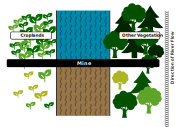
\includegraphics[width=\linewidth]{img/intro.pdf}
        \end{column}
    \end{columns}
\end{frame}

% ---------------------------------------------------


\begin{frame}{\textcolor{defaultclr!30}{Appendix}\hspace{0.75em}Basins}
\label{frame:appbasins}

\begin{columns}
    \begin{column}{0.4\textwidth}
        \centering
        \includegraphics[width=0.85\linewidth]{img/basins_lehnergrill.png}
        \textcolor{gray}{\footnotesize Illustration from \textcite{lehner2013}}
    \end{column}

    \begin{column}{0.55\textwidth}
        Our \textbf{unit of observation} is the \textbf{river basin}.

        \vspace{1em}

        \textcite{lehner2013} provide a nested basin collection, of which we use the \textbf{most granular level}.

        \vspace{1em}

        If we spill a cup of water anywhere in a basin, it always ends up in the next basin \colorbox{downcol!30}{\bfseries downstream}.

        \vspace{1em}\flushright

        \hyperlink{frame:intro}{\beamerbutton{\bfseries go back}}
    \end{column}
\end{columns}

\end{frame}

% ---------------------------------------------------
\begin{frame}{\textcolor{defaultclr!30}{Appendix}\hspace{0.75em}Intuition}
\label{frame:intu}
\begin{columns}
    \begin{column}{0.4\textwidth}
        The \textbf{four mines} depicted give an intuition for what we expect.

        \vspace{1em}

        Following the river “flow” from left to right, we can see \textbf{discontinuities} at the \textbf{mine basin}.
    \end{column}

    \begin{column}{0.55\textwidth}
        \centering
        \includegraphics[width=\linewidth]{img/mine-basin_ord-discont.pdf}
        \hyperlink{frame:appintu}{\beamerbutton{\bfseries show distance}} 
    \end{column}
\end{columns}

\end{frame}

% -------------------------------------------------

\begin{frame}{\textcolor{defaultclr!30}{Appendix}\hspace{0.75em}A Proxy for Agricultural Activity}

\begin{itemize}
    \item We get a \textbf{proxy} for \textbf{agricultural productivity} like this:

\begin{tcolorbox}[colback=ForestGreen!20, colframe=ForestGreen!20, fontupper=\color{ForestGreen!40!black}, width=\linewidth, sharp corners, boxrule=0pt]
\begin{enumerate}[(1)]
    \item Filter out \textbf{cloud cover}.
    \item Aggregate the \textbf{mean EVI} per basin.
    \item Take the \textbf{annual maximum} per basin per year. \colorbox{ForestGreen!80}{\bfseries\color{white} $\rightarrow$ Max. EVI}
    \item Apply a \textbf{cropland mask} \parencite{DigitalEarthAfrica2022}. \colorbox{ForestGreen!80}{\bfseries\color{white} $\rightarrow$ Max. Cropland EVI}
\end{enumerate}
\end{tcolorbox}

\vspace{0.5em}

\item This \textbf{Peak Vegetation Index} has been shown to proxy well for crop yields \parencite{azzari2017, beckerreshef2010, bolton2013, johnson2016}.
\end{itemize}
\end{frame}

% ---------------------------------------------------

\begin{frame}{\textcolor{defaultclr!30}{Appendix}\hspace{0.75em}Summary Statistics}
\label{frame:sumstats}
    \centering
    \renewcommand{\arraystretch}{1} 
    \rowcolors{2}{gray!15}{white}
    \begin{tabular}{lrrrrr} 
    \toprule \textbf{Variable} & \textbf{\textit{N}} & \textbf{Mean} & \textbf{St.~Dev.} & \textbf{Min.} & \textbf{Max.} \\ \midrule
    \textbf{Max.~EVI} & 114,616 & 0.411 & 0.168 & $-$0.112 & 0.993 \\ 
    \textbf{Mean EVI} & 114,616 & 0.270 & 0.118 & $-$0.112 & 0.578 \\ 
    \textbf{Max.~Cropland EVI} & 94,671 & 0.454 & 0.129 & $-$0.112 & 0.990 \\ 
    \textbf{Mean Cropland EVI} & 94,671 & 0.286 & 0.093 & $-$0.114 & 0.734 \\ 
    \textbf{Max.~Temperature} & 114,616 & 33.80 & 4.047 & 20.00 & 45.40 \\ 
    \textbf{Precipitation} & 114,616 & 882.3 & 606.3 & 0.555 & 4,375.3 \\ 
    \textbf{Population} & 114,536 & 8,185 & 37,090 & 0.000 & 1,396,921 \\ 
    \textbf{Elevation} & 114,616 & 804.6 & 482.0 & $-$118.3 & 3,059.7 \\ 
    \textbf{Slope} & 114,616 & 2.201 & 2.320 & 0.000 & 20.92 \\ 
    \textbf{Accessibility} & 114,576 & 183.9 & 255.9 & 1.002 & 7,681 \\  \bottomrule
    \end{tabular}
    \renewcommand{\arraystretch}{0.68}

    \vspace{0.5em}
    \hyperlink{frame:covars}{\beamerbutton{\bfseries go back to observations overview}} 
    \hyperlink{frame:covars_balance}{\beamerbutton{\bfseries show balance}}
\end{frame}


% ---------------------------------------------------


\begin{frame}{\textcolor{defaultclr!30}{Appendix}\hspace{0.75em}Order Specification Results}
\label{frame:orderapp}

\begin{itemize}
    \item We can see that \colorbox{upcol!30}{\bfseries upstream} basins are unaffected, while \colorbox{downcol!30}{\bfseries downstream} basins experience a significant negative effect.

    \vspace{1em} 

\item At the sample mean, the effect for the

\vspace{0.5em}

\begin{itemize}
    \item \colorbox{defaultclr!30}{\bfseries Max. EVI} corresponds to an EVI reduction of \textbf{1.4\%}.
    \vspace{0.25em}
    \item \colorbox{secondclr!30}{\bfseries Max. Cropland EVI} corresponds to an EVI reduction of \textbf{2.1\%}.
\end{itemize}

\vspace{1em} 

\item The effect \textbf{persists} beyond the mine basin.

\vspace{1em}

\item At higher order basins, impacts become imprecise.

\end{itemize}

\centering\hyperlink{frame:order}{\beamerbutton{\bfseries go back}}

\end{frame}

% ---------------------------------------------------


\begin{frame}{\textcolor{defaultclr!30}{Appendix}\hspace{0.75em}Impact Decay Assessment}
\label{frame:appdecay}
\begin{itemize}
    \item We re-estimate our main specification using an \textbf{exponential decay} function \(\exp\{-\delta \symrm{d}_{ij}\}\).
    \item \textbf{Hydrological studies} on dispersion patterns suggest using an exponential decay function.
    \item Since the \textbf{decay parameter} is not known, we conduct a grid search for \(\delta \in [0.001, 2]\).
    \item We then use a \textbf{Bayesian model averaging} approach with BIC as marginal likelihood approximation.
    \item Finally, we compute the \textbf{mean effect decay} at increasing distances.
\end{itemize}

  \centering\hyperlink{frame:decay}{\beamerbutton{\bfseries go back}} 
\end{frame}

% ---------------------------------------------------

\begin{frame}{\textcolor{defaultclr!30}{Appendix}\hspace{0.75em}Four Selected Mines, Distance}
\label{frame:appintu}
  \centering
  \includegraphics[width=.8\linewidth]{img/mine-basin_dist-discont.pdf}

  \hyperlink{frame:intu}{\beamerbutton{\bfseries go back}} 
\end{frame}

% ---------------------------------------------------

\begin{frame}{\textcolor{defaultclr!30}{Appendix}\hspace{0.75em}Basin Numbers}
\label{frame:appbasinno}
  \centering
  \includegraphics[width=.6\linewidth]{img/mine-basin_extents.png}
  
  \hyperlink{frame:covars}{\beamerbutton{\bfseries go back to observations overview}} 
\end{frame}

% ---------------------------------------------------

\begin{frame}{\textcolor{defaultclr!30}{Appendix}\hspace{0.75em}Basins by Order}
    \centering
    \begin{tabular}{rllll}
      \toprule Order & \multicolumn{2}{l}{Downstream} & \multicolumn{2}{l}{Upstream} \\
        & $N$ & Distance (km) & $N$ & Distance (km) \\ \midrule
      0 & 1900 & 0.0 & - & - \\ 
      1 & 1162 & 10.7 & 987 & 14.5 \\ 
      2 & 841 & 22.2 & 865 & 24.2 \\ 
      3 & 695 & 32.9 & 778 & 34.7 \\ 
      4 & 591 & 43.7 & 738 & 44.7 \\ 
      5 & 531 & 54.4 & 681 & 55.1 \\ 
      6 & 462 & 64.8 & 593 & 65.9 \\ 
      7 & 418 & 74.3 & 575 & 75.6 \\ 
      8 & 376 & 85.1 & 530 & 86.6 \\ 
      9 & 343 & 95.9 & 499 & 95.7 \\ 
      10 & 310 & 106.1 & 452 & 104.2 \\ \bottomrule
    \end{tabular}
    
    \vspace{0.5em}
    
    \hyperlink{frame:covars}{\beamerbutton{\bfseries go back to observations overview}} 
\end{frame}

% ---------------------------------------------------

\begin{frame}{\textcolor{defaultclr!30}{Appendix}\hspace{0.75em}Summary Statistics for Upstream Basins}
\label{frame:covars_balance}
    \centering
\begin{tabular}{@{\extracolsep{5pt}}lrrrrr} 
\toprule \multicolumn{6}{c}{Upstream Basins} \\ \midrule
Variable & $N$ & Mean & St.~Dev. & Min. & Max. \\ \midrule
Max. EVI & 53,584 & 0.417 & 0.169 & 0.021 & 0.983 \\ 
Mean EVI & 53,584 & 0.276 & 0.120 & 0.020 & 0.578 \\ 
Max. Cropland EVI & 44,389 & 0.459 & 0.127 & 0.057 & 0.990 \\ 
Mean Cropland EVI & 44,389 & 0.291 & 0.093 & $-$0.002 & 0.637 \\ 
Max. Temperature & 53,584 & 33.83 & 4.003 & 20.00 & 45.10 \\ 
Precipitation & 53,584 & 905.4 & 606.5 & 0.851 & 3,976.0 \\ 
Population & 53,584 & 6,693.8 & 27,878.2 & 0.000 & 1,396,921.0 \\ 
Elevation & 53,584 & 840.5 & 471.2 & 10.53 & 3,059.7 \\ 
Slope & 53,584 & 2.295 & 2.256 & 0.086 & 20.91 \\ 
Accessibility & 53,584 & 192.0 & 242.3 & 3.000 & 7,542.8 \\ \bottomrule
\end{tabular} 

\vspace{0.5em}

\hyperlink{frame:covars}{\beamerbutton{\bfseries go back to covariate overview}} 
\hyperlink{frame:sumstats}{\beamerbutton{\bfseries go back to summary statistics}}
\end{frame}

% ---------------------------------------------------

\begin{frame}{\textcolor{defaultclr!30}{Appendix}\hspace{0.75em}Summary Statistics for Downstream Basins}
    \centering
\begin{tabular}{@{\extracolsep{5pt}}lrrrrr} 
\toprule 
\multicolumn{6}{c}{Downstream Basins (incl. Mine Basins)} \\ \midrule
Variable & $N$ & Mean & St.~Dev. & Min. & Max. \\ \midrule
Max. EVI & 61,032 & 0.406 & 0.167 & $-$0.112 & 0.993 \\ 
Mean EVI & 61,032 & 0.264 & 0.116 & $-$0.112 & 0.563 \\ 
Max. Cropland EVI & 50,282 & 0.450 & 0.130 & $-$0.112 & 0.981 \\ 
Mean Cropland EVI & 50,282 & 0.283 & 0.093 & $-$0.114 & 0.734 \\ 
Max. Temperature & 61,032 & 33.78 & 4.085 & 20.00 & 45.40 \\ 
Precipitation & 61,032 & 862.0 & 605.4 & 0.555 & 4,375.3 \\ 
Population & 60,952 & 9,497.1 & 43,568.1 & 0.000 & 1,244,492.0 \\ 
Elevation & 61,032 & 773.1 & 489.1 & $-$118.3 & 3,047.1 \\ 
Slope & 61,032 & 2.119 & 2.371 & 0.000 & 20.456 \\ 
Accessibility & 60,992 & 176.9 & 267.1 & 1.002 & 7,681.8 \\ 
\bottomrule
\end{tabular} 

\vspace{0.5em}

 \hyperlink{frame:covars}{\beamerbutton{\bfseries go back to covariate overview}} \hyperlink{frame:sumstats}{\beamerbutton{\bfseries go back to summary statistics}}
\end{frame}

% ---------------------------------------------------

\begin{frame}{\textcolor{defaultclr!30}{Appendix}\hspace{0.75em}Full Order Specification Results}
\label{frame:orderfull}
 \centering

\begin{adjustbox}{width=0.45\textwidth, center}
   \begin{tabular}{lcccccc}\label{tab:app_main_order}
      \tabularnewline \midrule \midrule
      Dependent Variables: & \multicolumn{3}{c}{Maximum EVI} & \multicolumn{3}{c}{Maximum Cropland EVI}\\
      Model:                    & (1)             & (2)                     & (3)                            & (4)             & (5)                           & (6)\\  
      \midrule
      \emph{Variables}\\
      Downstream x Order $=$ 0  & -0.0064$^{***}$ & -0.0063$^{***}$         & -0.0059$^{***}$                & -0.0093$^{***}$ & -0.0097$^{***}$               & -0.0095$^{***}$\\   
                                & (0.0014)        & (0.0014)                & (0.0013)                       & (0.0021)        & (0.0021)                      & (0.0020)\\   
      Downstream x Order $=$ 1  & -0.0060$^{***}$ & -0.0048$^{***}$         & -0.0057$^{***}$                & -0.0049$^{*}$   & -0.0050$^{*}$                 & -0.0061$^{**}$\\   
                                & (0.0018)        & (0.0018)                & (0.0017)                       & (0.0026)        & (0.0027)                      & (0.0026)\\   
      Downstream x Order $=$ 2  & -0.0070$^{***}$ & -0.0053$^{**}$          & -0.0066$^{***}$                & -0.0042         & -0.0046                       & -0.0062$^{**}$\\   
                                & (0.0021)        & (0.0021)                & (0.0021)                       & (0.0028)        & (0.0029)                      & (0.0030)\\   
      Downstream x Order $=$ 3  & -0.0094$^{***}$ & -0.0069$^{***}$         & -0.0083$^{***}$                & -0.0049         & -0.0049                       & -0.0069$^{**}$\\   
                                & (0.0023)        & (0.0023)                & (0.0022)                       & (0.0032)        & (0.0033)                      & (0.0033)\\   
      Downstream x Order $=$ 4  & -0.0071$^{***}$ & -0.0053$^{**}$          & -0.0059$^{**}$                 & -0.0027         & -0.0036                       & -0.0044\\   
                                & (0.0025)        & (0.0024)                & (0.0024)                       & (0.0034)        & (0.0036)                      & (0.0036)\\   
      Downstream x Order $=$ 5  & -0.0077$^{***}$ & -0.0052$^{**}$          & -0.0056$^{**}$                 & -0.0009         & -0.0013                       & -0.0018\\   
                                & (0.0028)        & (0.0026)                & (0.0026)                       & (0.0037)        & (0.0038)                      & (0.0039)\\   
      Downstream x Order $=$ 6  & -0.0084$^{***}$ & -0.0054$^{*}$           & -0.0056$^{**}$                 & -0.0042         & -0.0044                       & -0.0051\\   
                                & (0.0031)        & (0.0028)                & (0.0028)                       & (0.0039)        & (0.0041)                      & (0.0041)\\   
      Downstream x Order $=$ 7  & -0.0093$^{***}$ & -0.0063$^{**}$          & -0.0063$^{**}$                 & 0.0008          & 0.0003                        & $-2.53\times 10^{-5}$\\    
                                & (0.0033)        & (0.0031)                & (0.0030)                       & (0.0041)        & (0.0043)                      & (0.0044)\\   
      Downstream x Order $=$ 8  & -0.0140$^{***}$ & -0.0110$^{***}$         & -0.0109$^{***}$                & -0.0074$^{*}$   & -0.0085$^{**}$                & -0.0090$^{**}$\\   
                                & (0.0033)        & (0.0031)                & (0.0031)                       & (0.0041)        & (0.0043)                      & (0.0044)\\   
      Downstream x Order $=$ 9  & -0.0103$^{***}$ & -0.0065$^{*}$           & -0.0067$^{**}$                 & -0.0042         & -0.0045                       & -0.0052\\   
                                & (0.0035)        & (0.0034)                & (0.0034)                       & (0.0039)        & (0.0043)                      & (0.0044)\\   
      Downstream x Order $=$ 10 & -0.0107$^{***}$ & -0.0056                 & -0.0056                        & -0.0038         & -0.0038                       & -0.0043\\   
                                & (0.0037)        & (0.0037)                & (0.0037)                       & (0.0045)        & (0.0049)                      & (0.0050)\\   
      Elevation                 &                 & $-7.77\times 10^{-6}$   & $-2.3\times 10^{-5}$$^{***}$   &                 & $-1.59\times 10^{-5}$$^{**}$  & $-3.86\times 10^{-5}$$^{***}$\\    
                                &                 & ($6.08\times 10^{-6}$)  & ($6.29\times 10^{-6}$)         &                 & ($7.19\times 10^{-6}$)        & ($7.35\times 10^{-6}$)\\    
      Slope                     &                 & 0.0034$^{***}$          & 0.0033$^{***}$                 &                 & 0.0023$^{***}$                & 0.0023$^{***}$\\   
                                &                 & (0.0005)                & (0.0005)                       &                 & (0.0006)                      & (0.0006)\\   
      Yearly Max. Temperature   &                 &                         & -0.0053$^{***}$                &                 &                               & -0.0071$^{***}$\\   
                                &                 &                         & (0.0007)                       &                 &                               & (0.0007)\\   
      Yearly Precipitation      &                 &                         & $3.33\times 10^{-5}$$^{***}$   &                 &                               & $2.86\times 10^{-5}$$^{***}$\\    
                                &                 &                         & ($3.61\times 10^{-6}$)         &                 &                               & ($3.95\times 10^{-6}$)\\    
      Accessibility in 2015     &                 &                         & $-9.97\times 10^{-6}$$^{*}$    &                 &                               & $-3.78\times 10^{-6}$\\    
                                &                 &                         & ($5.28\times 10^{-6}$)         &                 &                               & ($1.18\times 10^{-5}$)\\    
      Population in 2015        &                 &                         & $-1.51\times 10^{-7}$$^{***}$  &                 &                               & $-1.06\times 10^{-7}$$^{***}$\\    
                                &                 &                         & ($2.75\times 10^{-8}$)         &                 &                               & ($2.04\times 10^{-8}$)\\    
                                &                 &                         &                                &                 &                               &  \\  
      Sample Mean Effect        & -1.567          & -1.531                  & -1.438                         & -2.042          & -2.127                        & -2.089\\  
      \midrule
      \emph{Fixed-effects}\\
      Year                      & Yes             & Yes                     & Yes                            & Yes             & Yes                           & Yes\\  
      Mine                      & Yes             & Yes                     & Yes                            & Yes             & Yes                           & Yes\\  
      \midrule
      \emph{Fit statistics}\\
      Observations              & 114,616         & 114,616                 & 114,496                        & 94,671          & 94,671                        & 94,604\\  
      R$^2$                     & 0.91808         & 0.92156                 & 0.92395                        & 0.77981         & 0.78184                       & 0.78597\\  
      Within R$^2$              & 0.00393         & 0.04627                 & 0.05582                        & 0.00180         & 0.01099                       & 0.02531\\  
      \midrule \midrule
      \multicolumn{7}{l}{\emph{Clustered (Mine) standard-errors in parentheses}}\\
      \multicolumn{7}{l}{\emph{Signif. Codes: ***: 0.01, **: 0.05, *: 0.1}}\\
   \end{tabular}
\end{adjustbox}

\hyperlink{frame:order}{\beamerbutton{\bfseries go back}} 
    
\end{frame}


% ---------------------------------------------------

\begin{frame}{\textcolor{defaultclr!30}{Appendix}\hspace{0.75em}Full Distance Specification Results}
\label{frame:distfull}
 \centering

\begin{adjustbox}{width = 0.6\textwidth, center}
   \begin{tabular}{lcccccc}\label{tab:app_main_dist_squared}
      \tabularnewline \midrule \midrule
      Dependent Variables: & \multicolumn{3}{c}{Maximum EVI} & \multicolumn{3}{c}{Maximum Cropland EVI}\\
      Model:                            & (1)                     & (2)                     & (3)                            & (4)                           & (5)                           & (6)\\  
      \midrule
      \emph{Variables}\\
      Downstream                        & -0.0065$^{***}$         & -0.0060$^{***}$         & -0.0058$^{***}$                & -0.0086$^{***}$               & -0.0088$^{***}$               & -0.0087$^{***}$\\   
                                        & (0.0023)                & (0.0021)                & (0.0021)                       & (0.0029)                      & (0.0029)                      & (0.0028)\\   
      Downstream $\times$ Distance      & $-2.02\times 10^{-5}$   & $1.05\times 10^{-5}$    & $-2.02\times 10^{-5}$          & 0.0003$^{**}$                 & 0.0002$^{*}$                  & 0.0002\\   
                                        & (0.0001)                & (0.0001)                & (0.0001)                       & (0.0001)                      & (0.0001)                      & (0.0001)\\   
      Downstream $\times$ Distance$^2$  & $-3.98\times 10^{-7}$   & $-4.37\times 10^{-7}$   & $-9.8\times 10^{-8}$           & $-2.15\times 10^{-6}$$^{**}$  & $-2.34\times 10^{-6}$$^{**}$  & $-1.94\times 10^{-6}$$^{*}$\\    
                                        & ($9.17\times 10^{-7}$)  & ($7.35\times 10^{-7}$)  & ($7.19\times 10^{-7}$)         & ($1.06\times 10^{-6}$)        & ($1.03\times 10^{-6}$)        & ($1.03\times 10^{-6}$)\\    
      Distance                          & $4.05\times 10^{-5}$    & $2.98\times 10^{-5}$    & $2.56\times 10^{-5}$           & $-7.01\times 10^{-5}$         & $-5.62\times 10^{-5}$         & $-4.6\times 10^{-5}$\\    
                                        & ($9.03\times 10^{-5}$)  & ($8.4\times 10^{-5}$)   & ($8.19\times 10^{-5}$)         & (0.0001)                      & (0.0001)                      & (0.0001)\\   
      Distance$^2$                      & $-1.87\times 10^{-7}$   & $-9.18\times 10^{-9}$   & $2.1\times 10^{-8}$            & $6.93\times 10^{-7}$          & $8\times 10^{-7}$             & $6.06\times 10^{-7}$\\    
                                        & ($6.27\times 10^{-7}$)  & ($5.68\times 10^{-7}$)  & ($5.56\times 10^{-7}$)         & ($8.38\times 10^{-7}$)        & ($8.23\times 10^{-7}$)        & ($8.22\times 10^{-7}$)\\    
      Elevation                         &                         & $-7.45\times 10^{-6}$   & $-2.22\times 10^{-5}$$^{***}$  &                               & $-1.83\times 10^{-5}$$^{**}$  & $-4.03\times 10^{-5}$$^{***}$\\    
                                        &                         & ($6.56\times 10^{-6}$)  & ($6.71\times 10^{-6}$)         &                               & ($7.55\times 10^{-6}$)        & ($7.61\times 10^{-6}$)\\    
      Slope                             &                         & 0.0034$^{***}$          & 0.0032$^{***}$                 &                               & 0.0023$^{***}$                & 0.0023$^{***}$\\   
                                        &                         & (0.0005)                & (0.0005)                       &                               & (0.0006)                      & (0.0006)\\   
      Yearly Max. Temperature           &                         &                         & -0.0053$^{***}$                &                               &                               & -0.0070$^{***}$\\   
                                        &                         &                         & (0.0007)                       &                               &                               & (0.0007)\\   
      Yearly Precipitation              &                         &                         & $3.33\times 10^{-5}$$^{***}$   &                               &                               & $2.88\times 10^{-5}$$^{***}$\\    
                                        &                         &                         & ($3.6\times 10^{-6}$)          &                               &                               & ($3.94\times 10^{-6}$)\\    
      Accessibility in 2015             &                         &                         & $-1.01\times 10^{-5}$$^{*}$    &                               &                               & $-4.03\times 10^{-6}$\\    
                                        &                         &                         & ($5.31\times 10^{-6}$)         &                               &                               & ($1.19\times 10^{-5}$)\\    
      Population in 2015                &                         &                         & $-1.51\times 10^{-7}$$^{***}$  &                               &                               & $-1.06\times 10^{-7}$$^{***}$\\    
                                        &                         &                         & ($2.77\times 10^{-8}$)         &                               &                               & ($2.03\times 10^{-8}$)\\    
      \midrule
      \emph{Fixed-effects}\\
      Year                              & Yes                     & Yes                     & Yes                            & Yes                           & Yes                           & Yes\\  
      Mine                              & Yes                     & Yes                     & Yes                            & Yes                           & Yes                           & Yes\\  
      \midrule
      \emph{Fit statistics}\\
      Observations                      & 114,616                 & 114,616                 & 114,496                        & 94,671                        & 94,671                        & 94,604\\  
      R$^2$                             & 0.91804                 & 0.92152                 & 0.92390                        & 0.77971                       & 0.78175                       & 0.78587\\  
      Within R$^2$                      & 0.00346                 & 0.04573                 & 0.05524                        & 0.00138                       & 0.01060                       & 0.02485\\  
      \midrule \midrule
      \multicolumn{7}{l}{\emph{Clustered (Mine) standard-errors in parentheses}}\\
      \multicolumn{7}{l}{\emph{Signif. Codes: ***: 0.01, **: 0.05, *: 0.1}}\\
   \end{tabular}
\end{adjustbox}


\hyperlink{frame:dist}{\beamerbutton{\bfseries go back}} 
    
\end{frame}

% -------------------------------------------------

\begin{frame}{\textcolor{defaultclr!30}{Appendix}\hspace{0.75em}Varying Sample Definition}
\label{frame:sampledef}

\begin{adjustbox}{width = \textwidth, center}
   \begin{tabular}{lcccccccccc}\label{tab:rob_subsets_order}
      \tabularnewline \midrule \midrule
      Dependent Variables: & \multicolumn{5}{c}{Maximum EVI} & \multicolumn{5}{c}{Maximum Cropland EVI}\\
      Model: & (1) & (2) & (3) & (4) & (5) & (6) & (7) & (8) & (9) & (10)\\
      \midrule
      \emph{Variables}\\
      Downstream x Order $=$ 0 & -0.0059$^{***}$ & -0.0076$^{***}$ & -0.0062$^{***}$ &                 &                & -0.0095$^{***}$ & -0.0082$^{***}$ & -0.0094$^{***}$ &                &   \\   
                               & (0.0013)        & (0.0014)        & (0.0012)        &                 &                & (0.0020)        & (0.0024)        & (0.0022)        &                &   \\   
      Downstream x Order $=$ 1 & -0.0057$^{***}$ & -0.0053$^{***}$ & -0.0053$^{***}$ & -0.0049$^{**}$  & -0.0051$^{**}$ & -0.0061$^{**}$  & -0.0049         & -0.0051$^{*}$   & -0.0061$^{**}$ & -0.0069$^{*}$\\   
                               & (0.0017)        & (0.0020)        & (0.0017)        & (0.0020)        & (0.0021)       & (0.0026)        & (0.0032)        & (0.0030)        & (0.0030)       & (0.0039)\\   
      Downstream x Order $=$ 2 & -0.0066$^{***}$ & -0.0054$^{**}$  &                 & -0.0056$^{**}$  &                & -0.0062$^{**}$  & -0.0057         &                 & -0.0062$^{*}$  &   \\   
                               & (0.0021)        & (0.0026)        &                 & (0.0023)        &                & (0.0030)        & (0.0037)        &                 & (0.0033)       &   \\   
      \midrule
      \emph{Fixed-effects}\\
      Year                     & Yes             & Yes             & Yes             & Yes             & Yes            & Yes             & Yes             & Yes             & Yes            & Yes\\  
      Mine                     & Yes             & Yes             & Yes             & Yes             & Yes            & Yes             & Yes             & Yes             & Yes            & Yes\\  
      \midrule
      \emph{Fit statistics}\\
      Observations             & 114,496         & 61,712          & 32,360          & 99,320          & 9,168          & 94,604          & 50,914          & 27,589          & 81,278         & 7,623\\  
      R$^2$                    & 0.92395         & 0.91566         & 0.93993         & 0.92392         & 0.93378        & 0.78597         & 0.76613         & 0.84032         & 0.78332        & 0.81766\\  
      Within R$^2$             & 0.05582         & 0.05702         & 0.05650         & 0.05511         & 0.07364        & 0.02531         & 0.02382         & 0.03446         & 0.02322        & 0.03884\\  
      \midrule \midrule
      \multicolumn{11}{l}{\emph{Clustered (Mine) standard-errors in parentheses}}\\
      \multicolumn{11}{l}{\emph{Signif. Codes: ***: 0.01, **: 0.05, *: 0.1}}\\
   \end{tabular}
\end{adjustbox}


 \centering\hyperlink{frame:robust}{\beamerbutton{\bfseries go back}} 
    
\end{frame}

% -------------------------------------------------

\begin{frame}{\textcolor{defaultclr!30}{Appendix}\hspace{0.75em}Varying Outcome / Fixed Effects}
\label{frame:outfedef}

\begin{adjustbox}{width = \textwidth, center}
   \begin{tabular}{lccccccccc}\label{tab:rob_y-FE_order}
      \tabularnewline \midrule \midrule
      Dependent Variables: & \multicolumn{3}{c}{Maximum EVI} & Mean EVI & \multicolumn{3}{c}{Maximum Cropland EVI} & Mean C EVI & ESA C EVI\\
      Model: & (1) & (2) & (3) & (4) & (5) & (6) & (7) & (8) & (9)\\  
      \midrule
      \emph{Variables}\\
      Downstream x Order $=$ 0 & -0.0059$^{***}$ & -0.0065$^{***}$ & -0.0079$^{***}$ & -0.0048$^{***}$ & -0.0095$^{***}$ & -0.0104$^{***}$ & -0.0109$^{***}$ & -0.0073$^{***}$ & -0.0048$^{*}$\\   
                                & (0.0013)        & (0.0013)        & (0.0014)        & (0.0009)        & (0.0020)        & (0.0020)        & (0.0021)        & (0.0013)        & (0.0026)\\   
      Downstream x Order $=$ 1 & -0.0057$^{***}$ & -0.0060$^{***}$ & -0.0066$^{***}$ & -0.0035$^{***}$ & -0.0061$^{**}$  & -0.0062$^{**}$  & -0.0064$^{***}$ & -0.0043$^{**}$  & -0.0035\\   
                                & (0.0017)        & (0.0016)        & (0.0017)        & (0.0011)        & (0.0026)        & (0.0025)        & (0.0025)        & (0.0017)        & (0.0032)\\   
      Downstream x Order $=$ 2 & -0.0066$^{***}$ & -0.0064$^{***}$ & -0.0067$^{***}$ & -0.0038$^{***}$ & -0.0062$^{**}$  & -0.0058$^{**}$  & -0.0064$^{**}$  & -0.0055$^{***}$ & -0.0015\\   
                                & (0.0021)        & (0.0020)        & (0.0020)        & (0.0013)        & (0.0030)        & (0.0029)        & (0.0028)        & (0.0019)        & (0.0035)\\   
      \midrule
      \emph{Fixed-effects}\\
      Year                      & Yes             & Yes             & Yes             & Yes             & Yes             & Yes             & Yes             & Yes             & Yes\\  
      Mine                      & Yes             &                 &                 & Yes             & Yes             &                 &                 & Yes             & Yes\\  
      Pfaffstetter basin level 8&                 & Yes             &                 &                 &                 & Yes             &                 &                 & \\  
      Pfaffstetter basin level 6&                 &                 & Yes             &                 &                 &                 & Yes             &                 & \\  
      \midrule
      \emph{Fit statistics}\\
      Observations              & 114,496         & 114,496         & 114,496         & 114,496         & 94,604          & 94,604          & 94,604          & 94,604          & 67,649\\  
      R$^2$                     & 0.92395         & 0.91954         & 0.90419         & 0.95707         & 0.78597         & 0.77061         & 0.74193         & 0.88641         & 0.80154\\  
      Within R$^2$              & 0.05582         & 0.06500         & 0.08647         & 0.11783         & 0.02531         & 0.02957         & 0.04285         & 0.04478         & 0.02553\\  
      \midrule \midrule
      \multicolumn{10}{l}{\emph{Clustered (Mine) standard-errors in parentheses}}\\
      \multicolumn{10}{l}{\emph{Signif. Codes: ***: 0.01, **: 0.05, *: 0.1}}\\
   \end{tabular}
\end{adjustbox}



 \centering\hyperlink{frame:robust}{\beamerbutton{\bfseries go back}} 
    
\end{frame}

% ---------------------------------------------------

\begin{frame}{\textcolor{defaultclr!30}{Appendix}\hspace{0.75em}Placebo Outcomes}
\label{frame:placebo}
\begin{adjustbox}{width = \textwidth, center}
   \begin{tabular}{lcccccc}\label{tab:placebo_outcomes_quadratic}
      \tabularnewline \midrule \midrule
      Dependent Variables:              & Elevation      & Slope                   & Max. Temp               & Precipitation        & Accessibility in 2015 & Population in 2015\\  
      Model:                            & (1)            & (2)                     & (3)                     & (4)                  & (5)                   & (6)\\  
      \midrule
      \emph{Variables}\\
      Downstream                        & -6.852         & -0.0538                 & -0.0137                 & 0.6025               & -5.427                & 2,125.7\\   
                                        & (8.509)        & (0.0912)                & (0.0567)                & (3.934)              & (5.531)               & (1,589.8)\\   
      Distance $\times$ Downstream      & -5.008$^{***}$ & -0.0060                 & 0.0135$^{***}$          & -0.1942              & 0.0839                & -182.9$^{***}$\\   
                                        & (0.4814)       & (0.0044)                & (0.0036)                & (0.2860)             & (0.3278)              & (55.80)\\   
      Distance$^2$ $\times$ Downstream  & 0.0043         & $-8.25\times 10^{-6}$   & $2.12\times 10^{-6}$    & 0.0003               & 0.0004                & 1.081$^{***}$\\   
                                        & (0.0039)       & ($4.01\times 10^{-5}$)  & ($3.36\times 10^{-5}$)  & (0.0020)             & (0.0028)              & (0.3463)\\   
      Distance                          & 2.326$^{***}$  & 0.0025                  & -0.0067$^{**}$          & 0.0879               & 0.7557$^{***}$        & -54.72\\   
                                        & (0.4215)       & (0.0039)                & (0.0032)                & (0.2129)             & (0.2587)              & (45.17)\\   
      Distance$^2$                      & 0.0005         & $1.12\times 10^{-6}$    & $-5.34\times 10^{-6}$   & -0.0005              & -0.0013               & 0.3439\\   
                                        & (0.0033)       & ($3.49\times 10^{-5}$)  & ($3.1\times 10^{-5}$)   & (0.0015)             & (0.0021)              & (0.2724)\\   
      \midrule
      \emph{Fixed-effects}\\
      Year                              & Yes            & Yes                     & Yes                     & Yes                  & Yes                   & Yes\\  
      Mine                              & Yes            & Yes                     & Yes                     & Yes                  & Yes                   & Yes\\  
      \midrule
      \emph{Fit statistics}\\
      Observations                      & 114,616        & 114,616                 & 114,616                 & 114,616              & 114,576               & 114,536\\  
      R$^2$                             & 0.95627        & 0.70192                 & 0.95579                 & 0.96187              & 0.88768               & 0.59121\\  
      Within R$^2$                      & 0.41042        & 0.01108                 & 0.07605                 & 0.00070              & 0.04659               & 0.00851\\  
      \midrule \midrule
      \multicolumn{7}{l}{\emph{Clustered (Mine) standard-errors in parentheses}}\\
      \multicolumn{7}{l}{\emph{Signif. Codes: ***: 0.01, **: 0.05, *: 0.1}}\\
   \end{tabular}
   \end{adjustbox}

 \centering\hyperlink{frame:robust}{\beamerbutton{\bfseries go back}} 
    
\end{frame}



% ---------------------------------------------------

\begin{frame}{\textcolor{defaultclr!30}{Appendix}\hspace{0.75em}Dist. Spec. w/ Aut. Bandwith Selection (No Controls)}

\label{frame:autband}

% Table 1: No Controls
\centering
\begin{adjustbox}{width=0.8\textwidth}
\begin{tabular}{lcccc}
\toprule
& \multicolumn{2}{c}{\textbf{Max EVI}} & \multicolumn{2}{c}{\textbf{Max C EVI}} \\
\cmidrule(lr){2-3} \cmidrule(lr){4-5}
& \textbf{Conv.} & \textbf{Bias-Corr.} & \textbf{Conv.} & \textbf{Bias-Corr.} \\
\midrule
\multicolumn{5}{c}{\textbf{No Controls}} \\
\midrule
Conventional & -0.0050*** & -0.0056*** & -0.0112*** & -0.0116*** \\
& (0.0015) & (0.0015) & (0.0020) & (0.0025) \\
\midrule
Observations & 37,880 & 37,880 & 32,813 & 32,813 \\
Bandwidth (Conv) & 20.3 & 20.3 & 20.7 & 20.7 \\
Bandwidth (Bias) & 46.4 & 46.4 & 47.4 & 47.4 \\
\bottomrule
\end{tabular}
\end{adjustbox}

\vspace{3pt}

\scriptsize{
\textbf{Note:} Table shows results for estimation of \autoref{eq:main}, with distance as measured in kilometer along the river network used as the running variable, using practices suggested in \cite{cattaneo2019} for automatic bandwidth selection using a triangular Kernel and the mean squared error distance as selection criterion, and bias correction. Models in the upper panel include no covariates, models in the lower panel include the full set of controls. Models in columns (1) and (2) report results using the overall EVI as outcome, models in columns (3) and (4) for the cropland-specific EVI. Models (1) and (3) fit a linear polynomial of the distance measure at each side of the cutoff, models in columns (2) and (4) a quadratic polynomial. All specifications include mine and year fixed effects. Standard errors are clustered at the mine basin system level. \\
\textbf{Significance Codes:} *** p$<$0.01, ** p$<$0.05, * p$<$0.1 $\cdot$ Clustered (Mine) standard errors in parentheses.
}
\end{frame}

% ---------------------------------------------------

\begin{frame}{\textcolor{defaultclr!30}{Appendix}\hspace{0.75em}Dist. Spec. w/ Aut. Bandwith Selection (Full Controls)}
% Table 2: With Full Controls
\centering
\begin{adjustbox}{width=0.8\textwidth}
\begin{tabular}{lcccc}
\toprule
& \multicolumn{2}{c}{\textbf{Max EVI}} & \multicolumn{2}{c}{\textbf{Max C EVI}} \\
\cmidrule(lr){2-3} \cmidrule(lr){4-5}
& \textbf{Conv.} & \textbf{Bias-Corr.} & \textbf{Conv.} & \textbf{Bias-Corr.} \\
\midrule
\multicolumn{5}{c}{\textbf{With Full Controls}} \\
\midrule
Conventional & -0.0045*** & -0.0049*** & -0.0100*** & -0.0118*** \\
& (0.0015) & (0.0015) & (0.0020) & (0.0026) \\
\midrule
Observations & 38,200 & 38,200 & 32,629 & 32,629 \\
Bandwidth (Conv) & 20.6 & 20.6 & 20.5 & 20.5 \\
Bandwidth (Bias) & 43.4 & 43.4 & 45.4 & 45.4 \\
\bottomrule
\end{tabular}
\end{adjustbox}

\vspace{3pt}

\scriptsize{
\textbf{Note:} Table shows results for estimation of \autoref{eq:main}, with distance as measured in kilometer along the river network used as the running variable, using practices suggested in \cite{cattaneo2019} for automatic bandwidth selection using a triangular Kernel and the mean squared error distance as selection criterion, and bias correction. Models in the upper panel include no covariates, models in the lower panel include the full set of controls. Models in columns (1) and (2) report results using the overall EVI as outcome, models in columns (3) and (4) for the cropland-specific EVI. Models (1) and (3) fit a linear polynomial of the distance measure at each side of the cutoff, models in columns (2) and (4) a quadratic polynomial. All specifications include mine and year fixed effects. Standard errors are clustered at the mine basin system level. \\
\textbf{Significance Codes:} *** p$<$0.01, ** p$<$0.05, * p$<$0.1 $\cdot$ Clustered (Mine) standard errors in parentheses.
}
\end{frame}

% ---------------------------------------------------

\begin{frame}{\textcolor{defaultclr!30}{Appendix}\hspace{0.75em}Ord. Spec. w/ Aut. Bandwith Selection (Full Controls)}


\centering
\begin{adjustbox}{width=\textwidth}
\begin{tabular}{lcccc}
\toprule
& \multicolumn{2}{c}{\textbf{Max EVI}} & \multicolumn{2}{c}{\textbf{Max C EVI}} \\
\cmidrule(lr){2-3} \cmidrule(lr){4-5}
& \textbf{No Cluster} & \textbf{Cluster (Mine Basin)} & \textbf{No Cluster} & \textbf{Cluster (Mine Basin)} \\
\midrule
\multicolumn{5}{c}{\textbf{No Controls}} \\
\midrule
I(order$>$0) & -0.0048 & -0.0048 & -0.0090*** & -0.0090** \\
& (0.0013) & (0.0019) & (0.0018) & (0.0030) \\
\midrule
Observations & 45,613 & 45,613 & 38,537 & 38,537 \\
Bandwidth & 2 & 2 & 2 & 2 \\
\bottomrule
\end{tabular}
\end{adjustbox}

\vspace{0.5em}

\scriptsize{
\textbf{Note:} Table shows results for estimation of \autoref{eq:main}, with distance as measured by the ordering of basins with respect to the mine basin as the running variable, using practices suggested in \cite{kolesar2018} for automatic bandwidth selection using a triangular Kernel and the mean squared error distance as selection criterion. Models in the upper panel include no covariates, models in the lower panel include the full set of controls. Models in columns (1) and (2) report results using the overall EVI as outcome, models in columns (3) and (4) for the cropland-specific EVI. Models (1) and (3) do no cluster standard errors, models in columns (2) and (4) cluster standard errors are at the mine basin system level. All specifications include mine and year fixed effects. \\
\textbf{Significance Codes:} *** p$<$0.01, ** p$<$0.05, * p$<$0.1 
}

\end{frame}

% ---------------------------------------------------

\begin{frame}{\textcolor{defaultclr!30}{Appendix}\hspace{0.75em}Ord. Spec. w/ Aut. Bandwith Selection (Full Controls)}


\centering
\begin{adjustbox}{width=\textwidth}
\begin{tabular}{lcccc}
\toprule
& \multicolumn{2}{c}{\textbf{Max EVI}} & \multicolumn{2}{c}{\textbf{Max C EVI}} \\
\cmidrule(lr){2-3} \cmidrule(lr){4-5}
& \textbf{No Cluster} & \textbf{Cluster (Mine Basin)} & \textbf{No Cluster} & \textbf{Cluster (Mine Basin)} \\
\midrule
\multicolumn{5}{c}{\textbf{With Full Controls}} \\
\midrule
I(order$>$0) & -0.0048** & -0.0048 & -0.0090*** & -0.0090*** \\
& (0.0012) & (0.0018) & (0.0017) & (0.0029) \\
\midrule
Observations & 45,580 & 45,580 & 38,504 & 38,504 \\
Bandwidth & 2 & 2 & 2 & 2 \\
\bottomrule
\end{tabular}
\end{adjustbox}

\vspace{0.5em}

\scriptsize{
\textbf{Note:} Table shows results for estimation of \autoref{eq:main}, with distance as measured by the ordering of basins with respect to the mine basin as the running variable, using practices suggested in \cite{kolesar2018} for automatic bandwidth selection using a triangular Kernel and the mean squared error distance as selection criterion. Models in the upper panel include no covariates, models in the lower panel include the full set of controls. Models in columns (1) and (2) report results using the overall EVI as outcome, models in columns (3) and (4) for the cropland-specific EVI. Models (1) and (3) do no cluster standard errors, models in columns (2) and (4) cluster standard errors are at the mine basin system level. All specifications include mine and year fixed effects. \\
\textbf{Significance Codes:} *** p$<$0.01, ** p$<$0.05, * p$<$0.1 
}

\hyperlink{frame:robust}{\beamerbutton{\bfseries go back}} 
\end{frame}




% -------------------------------------------------



% ---------------------------------------------------
% END
% ---------------------------------------------------

\end{document}

% ---------------------------------------------------